\documentclass{article}
\usepackage[pdftex]{graphicx}
\begin{document}

\author{Jon Robison}
\title{CS595 Assignment 1}
\maketitle

Q1. Use curl to post to a web site
\begin{verbatim}
narfman0@fx3850 ~
$ curl "http://www.w3schools.com/html/html_form_action.asp?name=jrobison"
\end{verbatim}
\graphicspath{{q1/}}
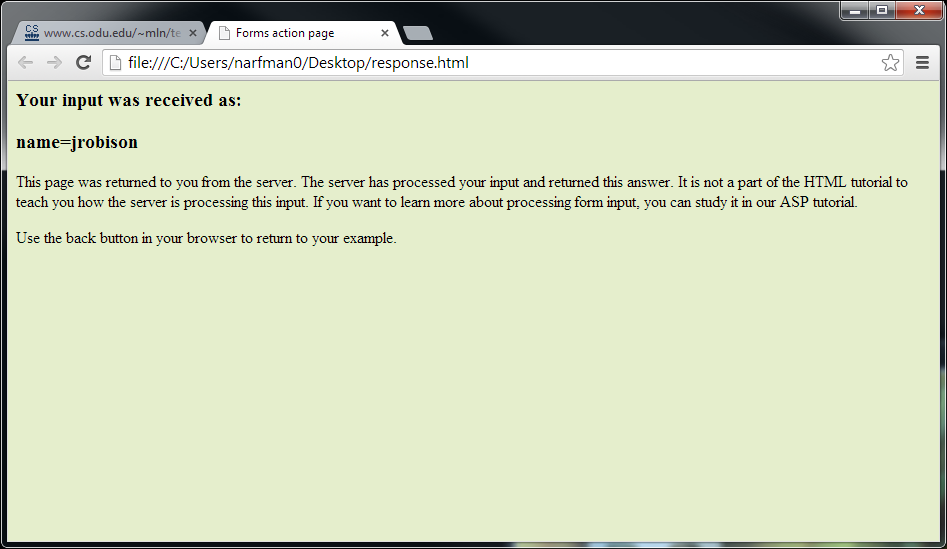
\includegraphics[scale=.4]{response.png}

Q2. Write a python score parser (code enclosed in q2/ScoreParser.py)
\begin{verbatim}
[narfman0@greeny q2]$ ./ScoreScanner.py "South Carolina" 5 "http://scores.espn.
go.com/ncf/scoreboard?confId=80&seasonYear=2013&seasonType=2&weekNumber=1"
South Carolina: 27 - North Carolina: 10
South Carolina: 27 - North Carolina: 10

[narfman0@greeny q2]$ ./ScoreScanner.py
Usage: ./ScoreScanner.py teamName waitTime uri
  Where teamName is your favorite team, e.g. South Carolina
    waitTime is a timeout between refreshing the scores, e.g. 5
    uri is the scores.espn.go.com child representing the database from 
which to draw, e.g. http://scores.espn.go.com/ncf/scoreboard?confId=80&
seasonYear=2013&seasonType=2&weekNumber=1
Since you left these arguments blank, assuming defaults
South Carolina: 27 - North Carolina: 10
South Carolina: 27 - North Carolina: 10
\end{verbatim}

Q3. Show bow-tie-edness of given graph
\begin{verbatim}
IN: I,L,M
SCC: A,B,C,G
OUT: D,H,K
Tendrils:
Tubes: J,N
Disconnected: E,F
\end{verbatim}
\end{document}